% c03：源文件 QuantumWorkTry.tex 第 938--1479 行
% 章节：第 2 节 2.1.8--2.3（APS 指标定理、反射正定性、拓扑超导体、其余情形概述）
% 说明：中文译注版正文片段；公式、编号、引用与原稿逐字对应

\subsubsection{APS 指标定理（The APS Index Theorem）}\label{aps}

在 \ref{why} 节中定义狄拉克指标 $\iota$ 时，我们用到如下事实：在可定向的四维流形上，狄拉克方程 $\D\psi=0$ 分解为分别关于 $\psi$ 的手征投影 $\psi_+$ 与 $\psi_-$ 的独立方程。

\begin{figure}[htbp]
  \centering
  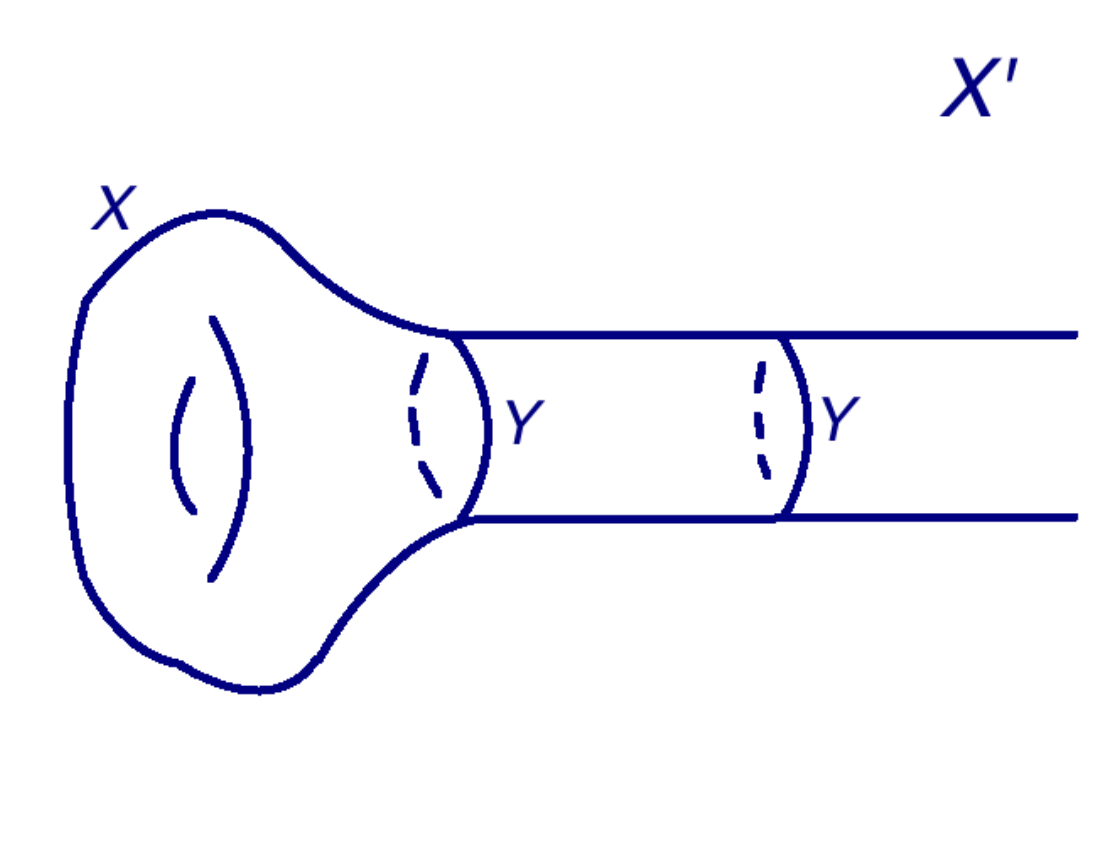
\includegraphics[width=0.55\textwidth]{fig06.png}
  \caption{完备而非紧致的流形 $X'$：在具有边界 $Y$ 的流形 $X$ 上黏接一根半无限长的管 $Y\times \R_+$ 而构成。（原文第 27 页，图 6）}
  \label{longer}
\end{figure}

APS 指标定理 \cite{APS} 是最初的 Atiyah--Singer 指标定理 \cite{ASfirst,AS} 向带边流形 $X$ 的推广。在试图寻求这一推广时，人们立即发现：沿 $Y=\partial X$ 并不存在一个便于用来定义指标的局部边界条件。狄拉克算子容许如下局部边界条件
\be\label{torz}\gamma\cdot n\,\psi=\pm \psi,\ee
其中 $n$ 是 $Y$ 的单位法向量，$\gamma\cdot n=\g^\mu n_\mu$。这一边界条件是保持边界局部旋转对称性的最一般条件；从物理上看它也合理，因为在此边界条件下狄拉克算子是厄米的。然而，由于 $\g\cdot n$ 与手征性算子 $\bg$ 反交换，这一边界条件混合了两种费米子手征性，因而无法用来定义狄拉克指标。

那么在此情形下应如何定义狄拉克指标呢？APS 的构造从如下做法开始：把带边流形 $X$ 替换为一个无边界、非紧致、但具有完备黎曼度量的流形 $X'$。具体做法是：在 $X$ 上（特别是在 $Y$ 上）选取黎曼度量，再沿 $X$ 的边界黏接一根半无限长的管 $Y\times \R_+$ 来构造 $X'$，其中 $\R_+$ 是半直线 $y\geq 0$（图 \ref{longer}）。管中的黎曼度量取为显然的 $\d y^2+g_Y$，其中 $g_Y$ 是 $Y$ 上选定的度量。

由于 $X'$ 没有边界，$X'$ 上的狄拉克方程不会混合正手征与负手征的旋量。因此可以定义 $X'$ 上狄拉克方程的\emph{平方可积}解所构成的空间 $H_+$ 与 $H_-$，它们分别由正、负手征性的解张成。其维数是整数 $n_+$ 与 $n_-$。暂设 $Y$ 的度量 $g_Y$ 足够一般，使 $Y$ 上的狄拉克算子 $\D_Y$ 没有零模。于是指标 $\iota$ 按通常方式定义为 $\iota=n_+-n_-$。

% [Tutor Note: 这里的指标就是狄拉克算子零模之差：$\iota$ 是 $X'$ 上正、负手征平方可积零模维数之差，与有限维线性代数中 $\dim\ker-\dim\coker$ 一致。之所以要求解「平方可积」，是因为 $X'$ 完备但非紧致；正是完备性保证谱离散、零模空间有限维，指标才有定义。原文紧接着用 $g_Y$ 的「一般性」假设避开 $\D_Y$ 的零模，否则 $\H_\pm$ 的划分本身不连续；后文说明该假设可以去掉。]

APS 指标定理给出 $\iota$ 的公式：
\be\label{trof}\iota=\hA-P-\frac{\etta}{2}. \ee
% [Tutor Note: 此处 $\hA-P$ 是四维 $\U(1)$ 规范场论中体贡献 $\int_X\hA(R)\,\tr\,e^F$ 的简写（$\hA$ 实指 $\int_X\hA(R)$，$P$ 为 $X$ 上的瞬子数，见本节后文与 \ref{why} 节）；$-\etta/2$ 才是 APS 定理相对 Atiyah--Singer 定理新增的边界项。$\etta$ 是 $Y$ 上狄拉克算子的 $\eta$ 不变量（定义见式（\ref{uv}）附近），它与后文整体反常分析中的 $\eta$ 相差因子 2：$\eta=2\etta$（见式（\ref{mold}））。理解本条的关键是：$\hA-P$ 与 $\etta/2$ 各自一般都不是整数，只有其组合 $\iota$ 是整数。]
其中 $\etta$ 是 $Y$ 上狄拉克算子 $\D_Y$ 的 $\etta$ 不变量（\ref{rv}）。于是 $-\etta/2$ 表现为对指标定理的一种边界修正。

对于无边界流形 $X$，狄拉克算子的指标是整数，而且是一个拓扑不变量。当 $X$ 有边界、指标以 APS 边界条件定义时，它仍然是整数，但不再是拓扑不变量。APS 指标公式清楚地表明了这一点。当 $X$ 与 $Y$ 上的度量和规范场变化到使 $\D_Y$ 的某个本征值穿过 0 时，$\etta$ 跳变 $\pm 2$，于是 $\iota$ 必须跳变 $\mp 1$。为具体理解这是如何发生的，我们考察管 $Y'=Y\times \R_+$ 中的狄拉克方程。$Y'$ 上的狄拉克算子 $\D_{Y'}$ 由 $\g_y$ 与 $\g_i$（$i=1,2,3$）定义：
\be \label{drowsy}\D_{Y'}=\i\left(\g^y\frac{\partial}{\partial y} +\sum_{i=1}^3 \g^i\frac{D}{D x^i}\right), \ee
其中 $x^i$（$i=1,\dots,3$）是 $Y$ 上的局部坐标。于是方程 $\D_{Y'}\psi=0$ 就是
\be\label{rowsy}\left(\frac{\partial}{\partial y}-\i\sum_{i=1}^3\i\g^y\g^i\frac{D}{D x^i}\right)\psi=0. \ee

我们希望用 $Y$ 上的狄拉克算子------它应为
\be\label{owsy}\D_Y=\i\sum_{i=1}^3\h\g^i \frac{D}{D x^i}. \ee
------来表示上式。这里 $\h \g_i$ 是纯三维的伽马矩阵，满足 $\{\h\g_i,\h\g_j\}=2g_{ij}$。在局部欧几里得标架中，可取它们为 $\h \g_i=\sigma_i$（其中 $\sigma_i$ 是泡利矩阵），从而满足 \be\label{blg}\h\g_1\h\g_2\h\g_3=\i\epsilon_{123}\ee（及其循环置换），其中 $\epsilon_{ijk}$ 是 $Y$ 的 Levi-Civita 张量。

% [Tutor Note: 由（\ref{drowsy}）到（\ref{rowsy}）只用了在方程两端左乘 $\i\g^y$ 并注意 $(\g^y)^2=1$、$\g^y$ 与 $\g^i$ 反交换：$\i\g^y\cdot\i\g^y\partial_y=-\partial_y$，$\i\g^y\cdot\i\g^i=-\g^y\g^i$，整理即得 $\partial_y\psi+\sum_i\g^y\g^i\frac{D}{Dx^i}\psi=0$。原文把系数 $+1$ 写成 $-\i\cdot\i$，于是（\ref{rowsy}）括号中出现「双重 $\i$」；若读者只数出一个 $\i$，就会把该项的符号弄反。]

在 $X$ 的手征性算子的定义（\ref{chiro}）中，我们取 $X$ 的定向使得 $\epsilon_{yijk}=\epsilon_{ijk}$。式（\ref{rowsy}）中出现的矩阵 $\g'_i=\i\g_y \g_i$ 满足与 $\h \g_i$ 相同的克利福德代数 $\{\g'_i,\g'_j\}=2g_{ij}$。它们在局部欧几里得标架中还满足 $\g'_1\g'_2\g'_3=\bg \cdot \i \epsilon_{123}$。由此可以推知，矩阵 $\bg \g'_i$ 满足与纯三维狄拉克矩阵 $\h\g_i$ 相同的克利福德代数以及相同的关系（\ref{blg}），因此可以令 $\bg\g'_i=\h\g_i$。于是我们可以把 $D=4$ 的狄拉克方程（\ref{rowsy}）改写为
\be\label{wsy}\left(\frac{\partial}{\partial y}-\bg\D_Y\right)\psi=0.\ee

% [Tutor Note: 「由此可以推知」省掉了克利福德代数在三维的唯一性定理：三个反交换、平方为 1 的矩阵在不可约表示中彼此只差一个整体符号（或置换），而（\ref{blg}）恰好把这个符号固定住；同时 $\bg\g'_i$ 也反交换且平方为 1，故 $\bg\g'_i=\h\g_i$ 相容。还需注意 $\bg$ 与 $\g'_i$ 反交换（$\bg$ 与每个 $\g^\mu$ 反交换），所以「把 $\bg$ 移过 $\g'_i$」会产生符号，这正是 $D=4$ 手征性算子作用在管上时的关键。]

于是，若 $\psi_0$ 是 $Y$ 上满足 $\D_Y\psi_0=\lambda\psi_0$ 的旋量场，并且 $\bg \psi_0=a\psi_0$（$a=\pm 1$），则可用
\be\label{syw}\psi =\exp(a\lambda y)\psi_0.\ee
求解 $D=4$ 的狄拉克方程。要得到该方程的平方可积解，当 $a=1$ 时需 $\lambda<0$，当 $a=-1$ 时需 $\lambda>0$。

现在来完成这一构造，说明原带边流形 $X$ 上的 APS 边界条件。设 $\H$ 为 $Y$ 上所有旋量场构成的空间，并作分解 $\H=\H_+\oplus \H_-$，其中 $\H_+$ 与 $\H_-$ 分别由 $\D_Y$ 的 $\lambda>0$ 与 $\lambda<0$ 的本征态张成。与通常一样，设 $\psi_+$ 与 $\psi_-$ 是四维旋量 $\psi$ 的正、负手征性部分。于是 $X$ 上的 APS 边界条件是说：$\psi_\pm$ 到 $Y=\partial X$ 的限制满足
\be\label{yw}\psi_+|_Y\in \H_-, ~~\psi_-|_Y\in\H_+. \ee
要点在于：$X$ 上狄拉克方程的解若能延拓为 $X'$ 上的平方可积解，当且仅当它满足这一条件。因此，我们既可以用 $X$ 上满足该 APS 边界条件的狄拉克方程的解，也可以用 $X'$ 上的平方可积解来计算指标 $\iota$。

% [Tutor Note: 注意（\ref{yw}）中「符号是反的」：正手征部分 $\psi_+$ 的边界值落在负本征值空间 $\H_-$ 中，负手征部分则落在 $\H_+$ 中。原因见（\ref{syw}）：对 $a=+1$（正手征）要使 $\exp(a\lambda y)$ 当 $y\to+\infty$ 时衰减，必须 $\lambda<0$。这正体现了 APS 边界条件是「非局部」的：它用 $Y$ 上整组本征模的谱分解来定义，而不是像（\ref{torz}）那样的逐点条件；也正因如此它才会混合手征性并依赖 $\D_Y$ 的谱。]

这就应当清楚地说明 $\iota$ 为何可能不是拓扑不变量。当 $\D_Y$ 的一个本征值穿过 0 时，空间 $\H_\pm$ 发生不连续的改变，APS 边界条件随之不连续地改变，指标 $\iota$ 也发生不连续的改变。

% [Tutor Note: $\etta$ 跳变 $\pm 2$ 与 $\iota$ 跳变 $\mp 1$ 的对应关系，可由 $\etta$ 的定义（\ref{uv}）逐项看出：单个本征值 $\lambda$ 从 $-\epsilon$ 变到 $+\epsilon$ 时，$\sign(\lambda)|\lambda|^{-s}$ 改变 $2|\lambda|^{-s}$，在 $s\to0$ 极限下贡献 $\pm2$；再由（\ref{trof}）即得 $\iota$ 的 $\mp1$ 跳变。物理图像是：每当 $Y$ 上出现一个零模，$X$ 中就有一个本征态在 APS 边界条件下「进出」正负手征空间，指标因而不可能对度规连续依赖。]

只要 $\D_Y$ 没有零模，$X$ 上带 APS 边界条件的狄拉克算子的谱就随 $X$（特别是随 $Y$）上的度量和规范场连续变化，而 $\iota$ 保持不变。在上文中，我们只在 $\D_Y$ 没有零模的一般情形下定义了 $\iota$、$\H_+$ 与 $\H_-$。对这些定义稍作修改，就能使 APS 指标公式（\ref{trof}）在一般情形下成立，其中 $\etta$ 用式（\ref{uv}）定义。

关于 APS 指标定理，我们还要再作几点说明。首先，式（\ref{trof}）中写出的是 $D=4$ 的 APS 指标定理。然而该定理对任意维数 $D$ 都成立。一般地，$\hA-P$ 须换为原来的 Atiyah--Singer 指标定理 \cite{ASfirst,AS} 所给出的体贡献（一般而言，该体贡献可写为 $\int_X\hA(R)\,\tr \,e^F$，其中 $F$ 是杨--米尔斯场强或曲率，迹取在费米子所属的表示中）。边界贡献始终是 $-\etta/2$。不过，当 $D$ 为奇数时，体贡献为零\footnote{原因仅仅在于 $R$ 与 $F$ 都是二形式，故 $\hA(R)\,\tr\,e^F$ 是偶数次形式的线性组合。若 $D$ 为奇数，则 $\hA(R)\,\tr\,e^F$ 没有 $D$ 次分量可以作为指标定理中的体贡献。}，APS 指标定理化为
% [Tutor Note: 原文此处疑有笔误（源第 1032--1034 行）：在「given by the original Atiyah-Singer index theorem \cite{ASfirst,AS} (this bulk contribution ... that the fermions live in.」一段中只有左括号而没有对应的右括号，系排印疏漏；译文按语义在「表示中」之后补出右括号，并以「边界贡献始终是 $-\etta/2$」接回正文。读者对照原文时不必以为此处有省略。]
\be\label{zolg} \iota=-\frac{\etta}{2}. \ee
由于 $\iota$ 总是整数，这表明：对奇数 $D$，若一个 $D-1$ 维流形 $Y$ 是某个 $D$ 维 $X$ 的边界，且相关结构可延拓到 $X$ 上（从而可在其上使用 APS 指标定理），则 $Y$ 上的 $\etta$ 不变量满足 $\etta/2\in\Z$。在后文关于马约拉纳费米子的应用中，我们将希望用 $\I=2\iota$、$\eta=2\etta$ 来写出这一公式：
\be\label{molg}\I=-\frac{\eta}{2}. \ee

% [Tutor Note: 由（\ref{zolg}）到（\ref{molg}）只做了变量替换 $\I=2\iota$、$\eta=2\etta$：$\I=2\iota=-\etta=-\eta/2$。这里 $2\iota$ 与 $2\etta$ 的因子并非笔误------马约拉纳费米子的本征值成对简并（见下文 Kramers 型论证），指标按「所有实零模」计数，恰为带电狄拉克费米子指标的两倍；$\eta$ 与「每对只取一个本征值」的受限和 $\etta$ 之差也恰为 2。]

APS 指标公式的另一重要推论，是 $\etta$ 与陈--西蒙斯函数
\be\label{zerf}\ICS(A)=\frac{e^2}{4\pi}\int_Y\,\d^3x \,\epsilon^{ijk}A_i\partial_jA_k. \ee
之间的关系。$\ICS(A)$ 只在模 $2\pi\Z$ 的意义下规范不变（这正是为什么在一切仅用 $A$ 的有效作用量描述的材料中，式（\ref{csm}）里的耦合常数 $k$ 必须是整数），但当 $A$ 连续变化时，它的变分 $\delta\ICS(A)$ 是完全规范不变的。若我们试图在其上定义 $\CS(A)$ 的自旋流形 $Y$ 是某个 $X$ 的边界（$A$ 与自旋结构均可延拓到其上），则
\be\label{xerf}\ICS(A)=2\pi P~{\mathrm{mod}}~2\pi\Z, \ee
其中 $P$ 是指标公式（\ref{trof}）中出现的、在 $X$ 上积分的瞬子数。该公式依赖于带边界 $Y$ 的四维自旋流形 $X$ 的选取方式，以及 $A$ 在 $X$ 上的延拓方式，但在模 $2\pi\Z$ 的意义下与这些选取无关。

为证明这一点，设 $X$ 与 $X'$ 是有相同边界 $Y$ 的自旋流形；$P$ 与 $P'$ 分别是 $X$ 与 $X'$ 上的瞬子数。则差 $P-P'$ 是整数，因为它等于在一个闭的可定向四维自旋流形 $\h X$ 上积分的瞬子数；$\h X$ 是把 $X'$ 黏接到 $X$ 上、再把 $X'$ 反向定向而成的（图 \ref{gluing}）。

\begin{figure}[htbp]
  \centering
  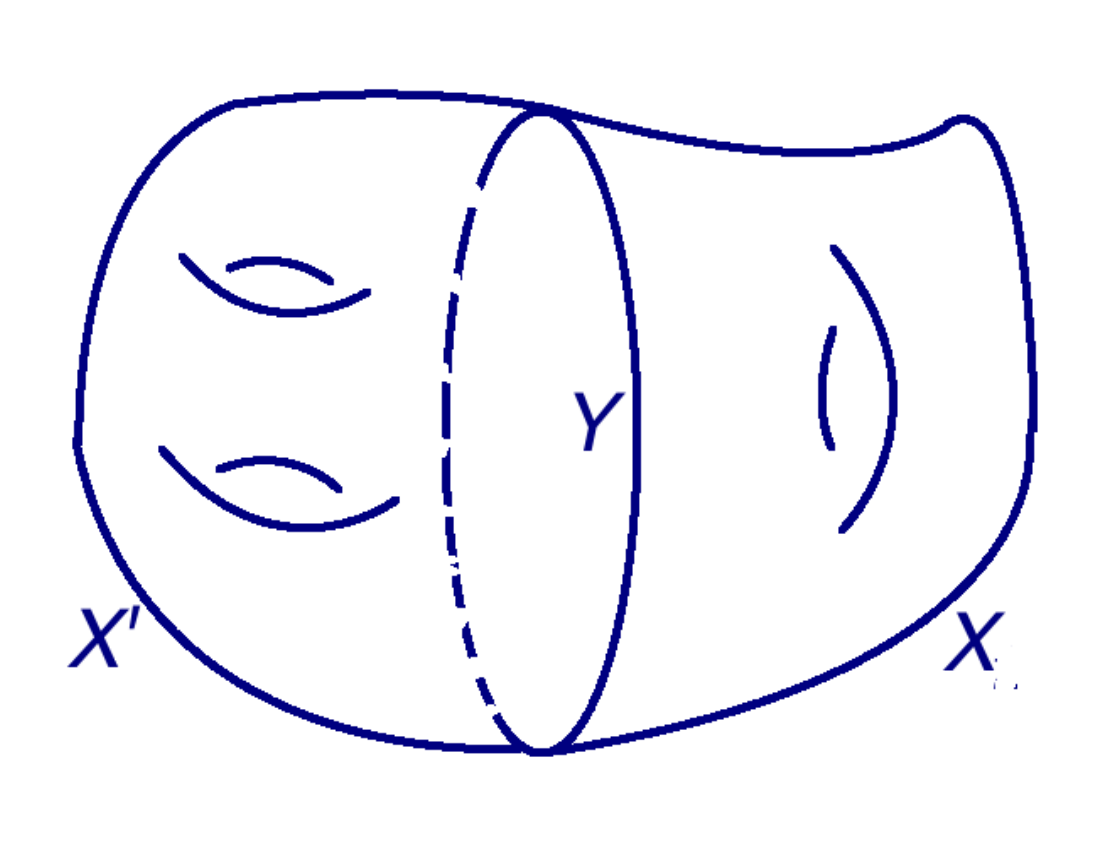
\includegraphics[width=0.55\textwidth]{fig07.png}
  \caption{把两个具有相同边界 $Y$ 的可定向四维流形 $X$ 与 $X'$ 黏接在一起（先反转 $X'$ 的定向，使两者的定向相容），便得到闭的可定向四维流形 $\h X$。若 $X$ 与 $X'$ 的自旋结构沿 $Y$ 一致，则 $\h X$ 是自旋流形。（原文第 31 页，图 7）}
  \label{gluing}
\end{figure}

类似地，可以定义一个引力陈--西蒙斯项 $\ICS_\grav$，它同样只在模 $2\pi\Z$ 的意义下有定义，并满足
\be\label{nerf}\ICS_\grav=2\pi \frac{\hA}{2}. \ee
（这里约定 $\hA$ 是在 $X$ 上积分的。公式用 $\hA/2$ 写出，是因为在无边界的四维自旋流形上 $\hA$ 为偶数。这一事实在 \ref{topsup} 节中很重要。）有了这些定义，并假定存在合适的 $X$，$X$ 上的 APS 指标定理就给出
\be\label{moj}\frac{\etta}{2}=\frac{\ICS(A)}{2\pi}-2\frac{\ICS_\grav}{2\pi}~~{\mathrm {mod}}~\Z. \ee
这一陈述只在模 $\Z$ 的意义下成立，因为它没有计入指标公式中的 $\iota$ 项。（此外，$\ICS(A)/2\pi$ 本身也只在模 $\Z$ 的意义下有定义，所以该陈述确实只在模 $\Z$ 的意义下有意义。）

% [Tutor Note: 把（\ref{xerf}）的 $\ICS(A)/2\pi\equiv P$ 与（\ref{nerf}）的 $\ICS_\grav/2\pi\equiv\hA/2$ 代入（\ref{trof}），得 $\etta/2=\hA-P-\iota$，故模 $\Z$ 有 $\etta/2\equiv\hA-P$；而（\ref{moj}）右端模 $\Z$ 为 $P-\hA$。两者相差 $2(\hA-P)$，是整数，故模 $\Z$ 之下并不矛盾------这正是原文声称「只到 mod $\Z$」的原因：符号约定在此精度下不可分辨。但若需要控制 $\exp(\mp\i\pi\etta/2)$ 的整体符号（下段马上要讨论的情形），就须把 $\etta/2$ 知道到 mod $2\Z$，此时（\ref{moj}）不够用。]

在导出 $\etta$ 与陈--西蒙斯的这一关系时，我们假定了所研究的流形 $Y$ 是某个 $X$ 的边界，且可在其上使用 APS 指标定理。若 $Y$ 是带 $\U(1)$ 规范场的三维自旋流形，这一点成立；但在我们可能应用 APS 指标定理的更一般问题中，它未必总成立。

即便如此，一个稍弱的陈述仍然成立。一般地，当 $Y$ 上的度量和规范场变化、并避开 $\etta$ 的跳变时，$\etta/2$ 与相应的陈--西蒙斯不变量之差是常数（但未必是整数）。为一般地陈述这一关系，设 $Y$ 的维数为 $d$，并一般地用 $\ICS(g,A)/2\pi$ 表示与指标定理中（$D=d+1$ 维）出现的曲率多项式\footnote{曲率多项式就是黎曼曲率 $R$ 与规范场场强或曲率 $F$ 的多项式。} $\hA\, \tr\,e^F$ 相关的陈--西蒙斯不变量（它推广了四维 $\U(1)$ 规范场论中的 $\hA-P$）。于是，在 $Y$ 上的度量和规范场 $(g,A)$ 作任意连续变化时，模去 $\etta$ 的偶数整数跳变，有
\be\label{noj}\frac{\delta\etta}{2}=\frac{\delta \ICS(g,A)}{2\pi}. \ee
这是把 APS 指标定理应用于 $D$ 维流形 $X=Y\times [0,1]$ 而证明的：其一端放一对场 $(g,A)$，另一端放一对略有不同的场 $(g',A')=(g+\delta g,A+\delta A)$。计入 $\etta$ 的跳变后，该陈述为
\be\label{oj} \frac{\etta}{2} =\frac{\ICS(g,A)}{2\pi}+{\mathrm{constant}}~~{\mathrm{mod}}~\Z.\ee
这个常数取值于 $\R/\Z$，在某些情形下是一个重要的拓扑不变量。它可以出现在整体反常中，因为整体反常与 $\etta$ 有关（\ref{complex} 节）。

在只关心模 $\Z$ 的 $\etta/2$、并假定 $X$ 存在（对三维自旋流形上的 $\U(1)$ 规范场论，它总是存在）的语境中，可以用式（\ref{moj}）把 $\etta$ 换成更初等的 $\ICS(A)$ 与 $\ICS_\grav$。然而，三维拓扑绝缘体的边界费米子具有配分函数 $Z_\psi=|Z_\psi| \exp(-\i\pi\etta/2)$，它依赖于模 $2\Z$（而非模 $\Z$）的 $\etta/2$。因此，替换（\ref{moj}）不足以描述这些边界费米子。若试图作此替换，我们就会失去对 $Z_\psi$ 整体符号的控制，而正如我们所看到的，这一符号对于描述拓扑绝缘体极为重要。

\subsubsection{反射正定性（Reflection Positivity）}\label{rpo}

另一个问题是：配分函数公式 $|Z_\psi|(-1)^\iota$ 为何与幺正性（即反射正定性）相容。

实际上，在眼下这一具体情形中，我们可以对这个疑问给出平凡的回答。我们把 $|Z_\psi|(-1)^\iota$ 构造为两个因子之积：$|Z_\psi|\exp(\mp \i\pi\etta/2)$ 与 $\exp(\pm \i\pi( P-\h A(R)))$。我们在关于图 \ref{dodo} 的讨论中已证明第一个因子是反射正定的；第二个因子也与反射正定性相容，否则规范与引力的 $\theta$ 角一般就不会在物理上合理。（具体地说，对任何实数 $\theta$，$\exp(\pm\i\theta (P-\h A(R)))$ 都与反射正定性相容，因为 $P$ 与 $\h A(R)$ 在反射下为奇，且对任何反射对称的规范场与度量都为零。）

\begin{figure}[htbp]
  \centering
  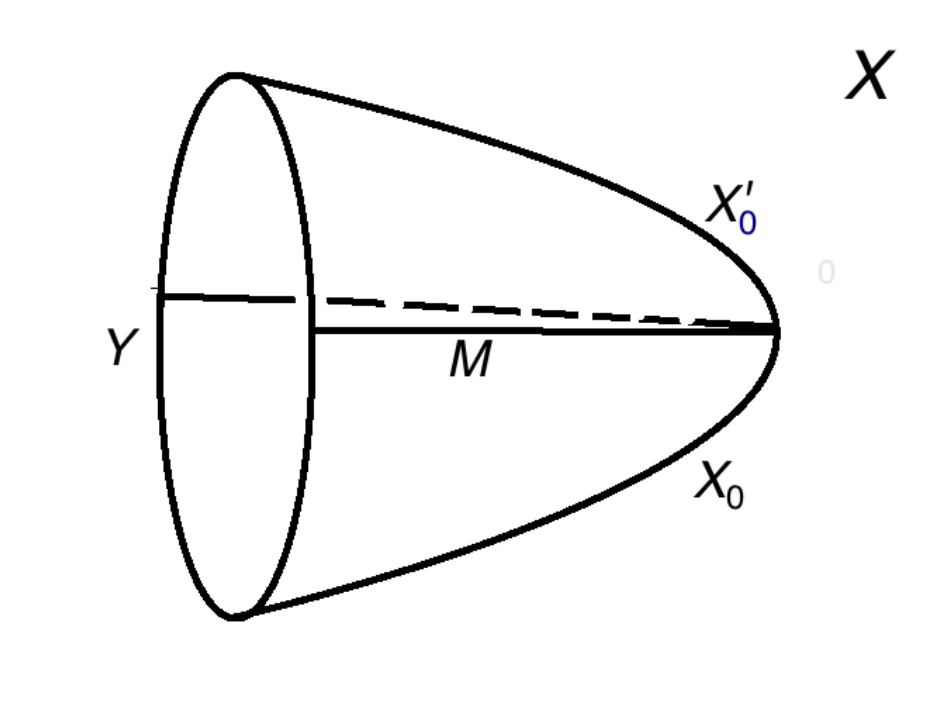
\includegraphics[width=0.55\textwidth]{fig08.png}
  \caption{一个有边界 $Y$ 的时空 $X$，它由某个流形 $X_0$ 的镜像副本黏接而成。图中这些副本记为 $X_0$ 与 $X_0'$。$Y$ 同样是镜像碎片的并集。$X_0$ 有两类边界：一类是 $M$，它沿此边界与 $X_0'$ 黏接；另一类是它与 $Y=\partial X$ 的交集。$X_0$ 在 $M\cap Y$ 处有角。（原文第 33 页，图 8）}
  \label{dodotwo}
\end{figure}

然而，着眼于其他情形，我们将直接证明 $|Z_\psi|(-1)^\iota$ 的反射正定性。我们要证明：只要一个带边界 $Y$ 的时空 $X$ 是沿公共边界 $M$ 把某个流形 $X_0$ 的两个镜像副本黏接而成（如图 \ref{dodotwo} 所示），$|Z_\psi|(-1)^\iota$ 就是实的且非负的。若 $X$ 有边界 $Y$，则此边界同样由镜像碎片黏接而成。此时 $X_0$ 实际上是带角的流形，如图所示。我们假定 $X$ 上的规范场、度量与自旋结构在交换 $X_0$ 的两个副本的反射下不变。

% [Tutor Note: 反射正定性的直接判据是：反射对称的配分函数须为实且非负。$\theta$ 角因子 $\exp(\pm\i\theta(P-\h A(R)))$ 之所以不破坏这一点，是因为 $P$ 与引力项 $\h A(R)$ 在反射下为奇（见 \ref{physical} 节关于 $P$ 为奇的讨论），反射对称的场组态使它们恰好为零，因子退化为 1；这也解释了为何 $\theta=\pi$ 这类「看似破坏 $\sT$」的角仍可与反射正定性相容，真正受限的是边界费米子的符号。后文说明：当 $X$ 由镜像双倍构造时，反射把正负手征互换，$D=4$ 的指标必然为零，于是 $(-1)^\iota=1$。另，下段原文（源第 1143 行）有笔误「they this boundary」，按上下文应为「then this boundary」，译文按其本意译出。]

由于 $|Z_\psi|$ 显然是实的且非负的，要证明 $|Z_\psi|(-1)^\iota$ 的反射正定性，只需证明在反射对称的情形下 $\iota=0$。反射会反转 $D=4$ 费米子的手征性，因此在任何反射对称的情形中，用 APS 边界条件算出的指标 $\iota$ 为零。证毕。

或者，我们也可以利用配边不变性来证明图 \ref{dodotwo} 情形中 $(-1)^\iota$ 的消失。这一解释的优点是：它几乎可以直接\footnote{要严格做到这一点，需要关于 $X_0$ 与 $X_0'$ 的自旋结构或 pin 结构的黏接的一些重要细节，这些细节是 D. Freed 告诉我的。在证明 $X$ 的自旋结构或 pin 结构可延拓到下文构造的流形 $Z$ 上时，必须用到这些细节。}推广到本文余下部分将要研究的其他例子，因为它们全都涉及配边不变的 sTQFT。若 $X$ 如图 \ref{dodotwo} 那样由某个流形 $X_0$「加倍」而成，则 $X$ 总是一个可以如下构造的流形 $Z$ 的边界。设 $M$ 是 $X_0$ 的边界中发生黏接的那一部分，如图所示。令 $Z_0=X_0\times I$，其中 $I$ 是单位区间 $[0,1]$，并在 $X_0$ 中把 $M\times I$ 收缩为 $M$。这样就得到一个以 $X$ 为边界的流形 $Z$。在 $M$ 附近的局部图像是：$Y$ 看起来像 $M\times \R_+$，$Z$ 看起来像 $M\times \R^2_+$，其中 $\R_+$ 与 $\R^2_+$ 分别是 $\R$ 或 $\R^2$ 中的半空间。$Z$ 的存在保证了 $X$ 的配边不变量（例如 $(-1)^\iota$）为零。

% [Tutor Note: 原文此处疑有笔误（源第 1164 行）：「Let $Z_0=X_0\times I$, ... and in $X_0$, collapse $M\times I$ to $M$.」按上下文，$M\times I$ 是 $Z_0=X_0\times I$ 的子集，应在 $Z_0$ 中收缩，而不是在 $X_0$ 中；译文照原文保留 $X_0$。这一「双倍--收缩」构造的本质是：把 $X_0\times I$ 中黏合面 $M$ 上的整段 $M\times I$ 捏成一点，使边界只剩 $X$，于是 $X=\partial Z$，配边不变量自然消失。]

\subsubsection{把故事倒过来讲（Running The Story In Reverse）}\label{reverse}

最后，把上述故事倒过来简述一遍也许会有启发。做法是：先在体中假设一个自旋拓扑量子场论（sTQFT），然后确定它可以具有何种保持对称性的边界态。

我们考虑一个带 $\U(1)$ 对称性的 $D=4$ sTQFT，其特征是：在紧致 $D=4$ 自旋流形 $X$ 上、在背景 $\U(1)$ 规范场 $A$ 存在时，其配分函数为 $(-1)^\iota$，其中 $\iota$ 是狄拉克算子的指标。它是 sTQFT 的配分函数，因为 Atiyah--Singer 指标定理表明 $\iota$ 是配边不变量，而一般地，这样的 $\U(1)$ 值配边不变量就是某个拓扑量子场论的配分函数。

拓扑绝缘体可以有空间边界；事实上在真实世界中------与思想实验不同------空间边界是不可避免的。因此我们希望把 sTQFT 推广到带边流形 $X$ 上。这并非易事。狄拉克算子的指标 $\iota$ 无法用 $\partial X$ 上的局部边界条件定义，但可以用整体的 APS 边界条件定义。然而如此定义的 $\iota$ 不是拓扑不变量；而且当背景数据（$X$ 上的度量和规范场）变化时，$\iota$ 会以非物理的方式跳变。

拓扑绝缘体的标准边界态是生活在 $\partial X$ 上的无质量狄拉克费米子。在这些模存在时，$\iota$ 的跳变在物理上是合理的。我们所描述的公式 $|Z_\psi|(-1)^\iota$ 是一个物理上合理的配分函数公式，适用于由体中的 sTQFT 与边界上的狄拉克费米子耦合而成的复合系统。$\iota$ 的跳变补偿了费米子配分函数符号定义中的困难。

\subsection{三维拓扑超导体（Topological Superconductor In $d=3$）}\label{topsup}

现在我们转向 $3+1$ 维的拓扑超导体，暂时只在可定向流形上表述。

\subsubsection{费米子与普法夫量（Fermions And Pfaffians）}\label{ferp}

拓扑超导体在体中是有能隙的（至少对费米型激发如此），但在边界上它支持一个两分量的马约拉纳费米子 $\psi$。与拓扑绝缘体分析的主要区别在于：$\psi$ 不带任何守恒荷（除 $(-1)^F$，即按模 2 计费米子数的算子之外）。特别地，与拓扑绝缘体相反，正电荷与负电荷的费米子模之间没有区别。这使得我们解释的细节需要作几处改动，尽管主要思想相同。由于费米子不携带守恒的可加荷，我们必须使用费米子的普法夫量（Pfaffian）而不是行列式。此外，我们还需要一个更细致的论证，来解释在 $\U(1)$ 不变情形下相当平凡的一个谱的二重化。

% [Tutor Note: 这里「没有守恒荷」是全文的枢纽：没有 $\U(1)$ 荷就无法把 $\psi$ 劈成 $\psi_+,\psi_-$ 两块，二次型不再能写成块反对角形式（\ref{wurmo}），于是路径积分只能是反对称双线性型的普法夫量而不能是行列式。反过来，一旦存在某个使 $\psi$ 劈裂的守恒荷，$\Pf$ 就化为 $\det$，见式（\ref{zurmo}）。]

洛伦兹号差下的三维马约拉纳费米子 $\psi$ 有 2 个实分量------它们按 $\Spin(1,2)\cong \SL(2,\R)$ 的实二维表示变换。延拓到欧几里得号差后，$\psi$ 仍有 2 个独立分量，尽管它们不再是实场；它们按 $\Spin(3)\cong \SU(2)$ 的二维赝实表示变换。（这不过是 $\SU(2)$ 的自旋 1/2 表示。）我们不能断言 $\psi$ 是实的，因为这与 $\SU(2)$ 对称性不相容；但尽管如此，$\psi$ 的复共轭并不出现在形式体系中。\footnote{这并不导致矛盾，因为费米子积分实际上是一种代数手续。我们对奇变量 $\psi$ 的定义是：$\int\d \psi\cdot 1=0$，$\int \d\psi\cdot\psi=1$，而从不需断言 $\psi$ 是实的，也不必提及它的复共轭。}因此，当我们写出 $\psi$ 作用量的欧几里得版本
\begin{equation}\label{zorb}I_\psi=\int\d^3x\,\bar\psi \DD \psi,  \end{equation}
时，尽管表面上如此，$\bar\psi$ 的定义中其实并不涉及复共轭。的确，对于延拓到欧几里得空间的马约拉纳费米子，定义就是 $\bar\psi_\alpha=\veps_{\alpha\beta}\psi^\beta$，其中 $\veps_{\alpha\beta}$ 是 $\Spin(3)=\SU(2)$ 不变的反对称张量。于是 $I_\psi$ 只是费米场 $\psi$ 的反对称双线性表达式。它之所以反对称，是由于费米统计。

仔细区分算子与双线性型是有益的。通常的厄米狄拉克算子 $\D=\i\slashed{D}=\i\sum_{i=1}^3\g^iD_i$ 是一个「算子」，概略地说就是 $\psi^\alpha\to \sum_\beta\i\slashed{D}^\alpha_\beta\psi^\beta$。$\psi^\alpha$ 的旋量指标可以用反对称张量 $\veps_{\alpha\beta}$ 升降；若这样做，就得到反对称双线性型 $\DD_{\gamma\beta}=\veps_{\gamma\alpha}\i\slashed{D}^\alpha_\beta$。

% [Tutor Note: 原文强调「并无复共轭」是针对形式体系而非物理：在欧几里得号差下 $\bar\psi_\alpha=\veps_{\alpha\beta}\psi^\beta$ 只是用 $\SU(2)$ 不变反对称张量把指标降下来。这一步把「厄米共轭」替换为「用 $\veps$ 缩并」，因此 $\bar\psi\DD\psi$ 是反对称双线性型而非厄米量；这也解释了为何 $Z_\psi$ 是 $\Pf$ 而非 $\det$ 的绝对值平方。若读者按洛伦兹号差的直觉把 $\bar\psi$ 当作 $\psi^\dagger\g^0$，就会误以为作用量不可能是反对称的。]

$\psi$ 场的路径积分在形式上就是这一反对称型的普法夫量：
\begin{equation}\label{turmo}Z_\psi=\Pf(\DD). \ee
凡是费米子理论，由于费米统计，费米作用量的二次部分总是反对称的，相应的费米路径积分就是作用量中出现的反对称双线性型的普法夫量。

什么时候可以说费米子的「行列式」而不是普法夫量呢？如果存在守恒的 $\U(1)$ 荷\footnote{只要存在使 $\psi$ 分解并产生类似式（\ref{wurmo}）结构的分解，$\U(1)$ 可以换成别的群。}，并且 $\psi$ 能分解为分别带正、负电荷的场 $\psi_+$ 与 $\psi_-$，就可以这样做。于是 $\U(1)$ 对称性保证：在基 $\bp \psi_+\cr \psi_-\ep$ 中，型 $\DD$ 是块反对角的
\begin{equation}\label{wurmo}\DD=\bp 0 & \D\cr -\D^\tr & 0 \ep. \ee
这里 $\D$ 不受任何对称或反对称条件限制，$\D^\tr$ 是它的转置。在这种情况下，有
\begin{equation}\label{zurmo}\Pf(\DD)=\det(\D),\ee
于是费米路径积分可以写成一个行列式。

回到马约拉纳费米子的厄米狄拉克算子 $\D$，由于 Kramers 二重化的一个欧几里得类比，它的本征值具有偶数重数。\footnote{导致三维时空中 $c$ 数模的这一欧几里得版 Kramers 二重化的数学事实，与导致 $3+1$ 维量子态通常的 Kramers 二重化的数学事实相同。一个不那么内蕴、但可能更眼熟的 $\mathcal T$ 的定义见附录 \ref{wwod}；参见式（\ref{zork}）。}若 $c$ 数旋量 $\chi$ 是狄拉克算子的本征向量，
\be\label{dolf}\D\chi=\lambda\chi,~~\lambda\in\R,\ee
则由 $\t\chi^\alpha=\veps^{\alpha\beta}\chi^*_\beta$ 定义的 $\t\chi$ 是同一本征值的本征向量
\be\label{old}\D\t\chi =\lambda\t\chi.\ee
这里 $\chi^*_\beta$ 表示 $\chi^\beta$ 的复共轭。尽管欧几里得场论中没有场对应于 $\psi$ 的复共轭，但当我们把 $\psi$ 按 $\D$ 的本征模展开、作为执行泛函积分的一步时，考察这些本征模在复共轭下的行为是有意义的。若用\be\label{norg}(\T\chi)^\alpha =\veps^{\alpha\beta}\chi^*_\beta,\ee
定义旋量上的反线性运算 $\T$，则 $[\T,\D]=0$ 且 $\T^2=-1$。正如 $3+1$ 维 Kramers 二重化的研究一样，这意味着 $\D$ 的本征值具有偶数重数。对赝实费米子，出于同样的理由，谱的二重化总是发生。只需把 $\veps^{\alpha\beta}$ 换成相应情形中有关的、不变反对称双线性型即可。

% [Tutor Note: $\T$ 是反线性算子（$\T(c\chi)=c^*\T\chi$），$\T^2=-1$ 才是 Kramers 型简并的根源：若 $\chi$ 与 $\T\chi$ 线性相关，则 $\chi=c\,\T\chi$，迭代得 $\chi=|c|^2\T^2\chi=-|c|^2\chi$，矛盾。原文「由于存在反线性对称性…因此本征模二重化」省掉了这一标准论证。注意对 4 维旋量（$\Spin(4)$ 旋量表示赝实）同一论证给出 $\I$ 为偶数，这是后文（\ref{neft}）处关键的一步。]

设 $\chi$ 与 $\T\chi$ 是 $\D$ 的一对同本征值 $\lambda$ 的本征模。由于定义 $\DD_{\g\beta}=\veps_{\g\alpha}\D^\alpha_\beta$，在以 $\bp \chi\cr\T\chi\ep$ 为基的 $2\times 2$ 块中，$\DD$ 取形式
\be\label{tf}\DD=\bp 0 & -\lambda \cr \lambda & 0 \ep.\ee
更一般地，考虑由 $\D$ 的形如 $\chi_i,\T\chi_i$ 的本征模组成的基（其中对 $i\not=j$，$\chi_i,\,\T\chi_i$ 与 $\chi_j,\,\T\chi_j$ 正交）。在这样的基中，$\DD$ 是块对角的，各 $2\times 2$ 块形如（\ref{tf}）。于是，$\DD$ 的普法夫量在形式上是
\be\label{rf} \Pf(\DD)=\prod_i{}'\,\lambda_i, \ee
其中乘积遍历 $\D$ 的本征值，符号 $\prod{}'$ 表示乘积中每一对只取一个本征值。

% [Tutor Note: 由块（\ref{tf}）可见每个 $2\times2$ 块的 $\Pf$ 恰为该块的 $\lambda$（$\Pf\bp 0&-\lambda\cr\lambda&0\ep=\lambda$）；块对角矩阵的 $\Pf$ 为各块 $\Pf$ 之积，故得（\ref{rf}）。注意这里有两个技术隐患，原文以「形式上」一词带过：(1) 乘积是无穷乘积，需要正规化（下文用 Pauli--Villars 的（\ref{polk}）实现）；(2) 若某一对本征值的 $\lambda=0$，则 $\Pf=0$，这正是「零模使符号无定义」的来源。另，原文（源第 1271 行）紧接上文作「More generally,,」，逗号重复，系排印疏漏，译文不复现该重复。]

让我们把这一点与狄拉克费米子的相应公式（\ref{peto}）作比较。在（\ref{peto}）左端，我们写的是 $\det\,\D$ 而不是 $\Pf(\DD)$，这反映了在 $\U(1)$ 不变情形下 $\Pf(\DD)$ 可写成 $\det\,\D$ 这一事实。在式（\ref{peto}）右端，本征值乘积只遍历正电荷费米子的本征值。（在该推导中，$\D$ 定义为作用在狄拉克费米子 $\psi$ 上的厄米狄拉克算子，而所谓狄拉克费米子是指具有确定电荷的费米子，不妨视为带正电荷。）由狄拉克方程的电荷共轭对称性，相应的带负电荷费米子具有完全相同的本征值，但式（\ref{peto}）没有计入它们。在马约拉纳情形中，我们借助 $\T^2=-1$ 这一事实、经由一个相对微妙的论证得到的狄拉克本征值二重化，在狄拉克情形中则更为平凡：它只不过意味着正、负电荷费米子的本征值相同。对任何赝实费米子系统都可以写出类似（\ref{rf}）的公式；当存在适当的对称性时，它就化为类似（\ref{peto}）的东西。

\subsubsection{谱流的消失（Vanishing Of The Spectral Flow）}\label{specvan}

现在来考虑 $\DD$ 的符号。正如拓扑绝缘体的讨论中那样，定义形式表达式（\ref{rf}）的符号可能存在一个问题，因为有无穷多对本征向量具有 $\lambda<0$。在给定的三维流形 $Y$ 上，我们可以从某个特定的度量 $g_0$ 出发，随意定义 $\Pf(\DD)$ 的符号，然后通过计数有多少对本征值对穿过 $\lambda=0$ 来在度量变化时演化这个符号。要判断这一手续给出的答案是否在与恒等元不连通的微分同胚下不变，就沿用 \ref{trada} 节中所述的映射环面方法。我们考虑与图 \ref{flow} 中相同的谱流问题，并问：穿过 $\lambda=0$ 的本征值对的数目 $\Delta$ 是偶数还是奇数。

结果 $\Delta$ 总是为零。证明的步骤如下。首先，我们在解释式（\ref{worf}）时提到的谱流论证 \cite{APS,DCG,Kiskis} 对马约拉纳费米子同样有效。差别仅在于：(1) 当没有 $\U(1)$ 对称性时，谱流 $\Delta$ 应定义为穿过 $\lambda=0$ 的本征值对的数目，而不是穿过 $\lambda=0$ 的正电荷本征值的数目；(2) 同样，当没有 $\U(1)$ 对称性时，我们必须用在整个费米子场空间中算出的 $D=4$ 狄拉克指标 $\I$ 来表达 $\Delta$，而不是只用正电荷费米子空间中的指标 $\iota$。两类指标（当两者都有定义时）之间的关系就是
\be\label{reft} \I=2\iota,\ee
因为电荷共轭意味着带负电荷费米子的 $D=4$ 指标与带正电荷费米子的相同。于是，式（\ref{worf}）在不假定 $\U(1)$ 对称性时仍然成立的推广是
\be\label{neft}\Delta =\frac{\I}{2}. \ee
这个公式有意义，因为在 $D=4$ 中 $\I$ 总是偶数\footnote{这一断言可用一个与我们在 $d=3$ 时证明狄拉克谱二重化所用论证类似的论证来证明。$\Spin(4)$ 的旋量表示是赝实的，因此 $D=4$ 中马约拉纳费米子的本征模由于存在反线性对称性 $(\T\chi)^\alpha=\veps^{\alpha\beta}\chi^*_\beta$、$\T^2=-1$、$[\T,\D]=0$ 而二重化。正、负手征性的零模都由这一论证二重化，因此 $\I$ 为偶数。}，这一事实在后续讨论中很重要。类似地，（\ref{torf}）的类比是：费米路径积分在微分同胚 $\phi$ 下的变换为
\be\label{weft}\Pf(\DD)\to \Pf(\DD)(-1)^{\I/2}. \ee
这里 $\I$ 是由 $\phi$ 构造的映射环面上狄拉克算子的指标，计入所有费米子。

% [Tutor Note: 「$\Delta$ 总是为零」并非初等事实，它依赖三件事：(i) APS 与 \cite{DCG,Kiskis} 关于谱流与指标关系的定理在无 $\U(1)$ 情形下的推广；(ii) 马约拉纳本征值成对出现（$\T^2=-1$），故谱流按「对」计数；(iii) 映射环面上的 $D=4$ 指标 $\I$ 恒为零（见下文脚注关于符号差的论证）。原文以一句「It turns out」跳过了 (i) 中「推广为何成立」的细节：实质上是把 $\U(1)$ 带电扇区的指标换成全费米子空间的指标，因子 2 由（\ref{reft}）补偿。]

这个公式不仅限于单个马约拉纳费米子只与引力耦合的情形。它适用于（在可定向三维流形上；不可定向情形留到 \ref{complex} 节）任何按任意紧致规范群的实表示变换的三维马约拉纳费米子系统。在许多情形中（例如拓扑绝缘体，此时式（\ref{weft}）等价于式（\ref{torf}）），该公式意味着 $\Pf(\DD)$ 的符号存在反常。然而，对单个只与引力耦合的马约拉纳费米子，并不存在这种反常。尽管在无边界紧致 $D=4$ 自旋流形上 $\I/2$ 一般可以取奇数\footnote{例如，在 K3 曲面上 $\I/2=1$。}，但在映射环面上它总是为零。\footnote{证明方法之一是注意到：在四维中，只与引力耦合的马约拉纳费米子的狄拉克指标与符号差 $\sigma$ 由 $\I=\sigma/8$ 相联系。但对任意维数的映射环面，一个相对初等的拓扑论证表明 $\sigma=0$。设 $X\to S^1$ 是一个映射环面，维数为 $4n$（$n$ 为某整数），纤维 $Y$ 的维数为 $4n-1$。考虑由形如 $W\times p$ 的闭链生成的子空间 $\Gamma\subset H_{2n}(X;\Z)$，其中 $W\subset Y$，$p$ 是 $S^1$ 中的一点。模去挠部分，$\Gamma$ 是 $H_{2n}(X;\Z)$ 上相交配对的一个零子空间。（对任意 $W,W'\subset Y$，$W\times p$ 与 $W'\times p$ 的相交数为 0，因为 $W'\times p$ 同调于 $W'\times p'$，其中 $p'\not= p \in S^1$，而 $W'\times p'$ 与 $W\times p$ 不相交。）可以用 Poincar\'e 对偶证明 $\Gamma$ 是中间维的。$H_{2n}(X;\Z)$ 模去挠部分存在中间维零子空间，就表明 $X$ 的符号差为 0。}

\subsubsection{路径积分的符号（The Sign Of The Path Integral）}\label{signp}

最后这句话意味着：在通常意义上，对于只与引力耦合的三维马约拉纳费米子，在可定向三维流形 $Y$ 上，$\Pf(\DD)$ 没有反常：在某个起始度量 $g_0$ 处随意选定其符号后，可以以一种在保向微分同胚下不变的方式对所有度量一致地定义该符号。然而，对每个 $Y$ 都允许路径积分有一个任意的独立符号，在物理上并不令人满意。正如 \ref{trada} 节中已经提到的，理论的满意定义应当与切割和黏接的物理要求相容地确定所有 $Y$ 上路径积分的相位。

% [Tutor Note: 这里区分了「无反常」与「无歧义」两件事：无反常只意味着符号可以沿度规空间一致地传播（单值、在保向微分同胚下不变），但每个连通的三维流形 $Y$ 仍可各自独立地选取初始符号；真正要构造的是所有 $Y$ 上一族彼此相容的符号，这正是下一段所说的「物理上自然的手续」。这一区分在拓扑绝缘体与拓扑超导体的讨论中都反复出现。]

现在我们要说明：尽管在通常意义上没有反常，但要以一种对所有 $Y$ 都一致的方式定义 $2+1$ 维马约拉纳费米子的费米路径积分，一个物理上自然的手续会导致 $\sT$ 与 $\sR$ 对称性的破坏，正如拓扑绝缘体所发生的那样。此外，在这一手续的框架内将会清楚：尽管 $(-1)^{\I/2}=1$ 对映射环面成立，但 $(-1)^{\I/2}\not=1$ 对某些其他（紧致、闭、可定向自旋的）流形成立这一事实，构成了一个障碍，使我们无法在不与体拓扑超导体耦合的情况下、以 $\sT$ 不变的方式单独定义 $2+1$ 维马约拉纳费米子。把与体的耦合包括进来，我们就会得到一个良定义且 $\sT$ 不变的答案。

尽管我不声称有形式证明，但可以预期，任何其他精确地为所有 $Y$ 定义 $2+1$ 维马约拉纳费米子配分函数的手续都会导致相同的结论。一般地，人们预期同一理论的两种合理正规化相差一个局部抵消项，但不存在能改变我们结论的局部抵消项。

为定义 $2+1$ 维马约拉纳费米子，我们将使用与狄拉克费米子相同的泡利--维拉尔斯正规化。费米子行列式的式（\ref{pv}）对应的普法夫量类比是
\be\label{polk}\Pf(\DD)_\reg=\prod_k{}'\frac{\lambda_k}{\lambda_k\pm\i\mu},\ee
其中正规化子质量的两个符号都允许。导致（\ref{yv}）的那些步骤现在给出马约拉纳费米子的路径积分
\be\label{oldo}Z_\psi=|Z_\psi| \exp(\mp\i\pi\etta/2),\ee
其中现在可以把 $\etta$ 定义为受限求和
\be\label{riv}\etta=\lim_{s\to 0}\sum_k{}'\sign(\lambda_k)|\lambda_k|^{-s} \ee
只计入每一对中的一个本征值。然而，更惯常的做法是把 $\eta$ 不变量定义为对所有本征值求和
\be\label{roov}\eta=\lim_{s\to 0}\sum_k\sign(\lambda_k)|\lambda_k|^{-s} ,\ee
于是 \be\label{mold}\eta=2\etta,\ee
并且应将费米子路径积分写为
\be\label{zold}Z_\psi=|Z_\psi|\exp(\mp \i\pi \eta/4).\ee

% [Tutor Note: 务必分清 $\etta$ 与 $\eta$：$\etta$ 是「每对只取一个本征值」的受限和，$\eta$ 是遍历全部本征值的和，故 $\eta=2\etta$；代入（\ref{oldo}）便得（\ref{zold}）中的 $\eta/4$。这个因子 4 是后文（\ref{wizont}）能与 $\hA(R)/2$ 配平的根源，也是最易出的错。另注意（\ref{polk}）中正规化子质量写成 $\pm\i\mu$，两个符号给出 $Z_\psi$ 的 $\mp$ 号；这一符号是正规化子的人为选择，正是它导致单独看 $Z_\psi$ 时 $\sT$ 破坏、需由体项补偿。]

这是破坏 $\sT$ 的，因为它不是实的；但正如 \ref{topthree} 节中那样，只要假定承载无质量马约拉纳费米子的三维流形 $Y$ 实际上是某个拓扑超导体的世界体 $X$ 的边界，我们就可以恢复 $\sT$ 不变性。拓扑超导体的显著性质是：在大体积极限下，它在无边界的闭（可定向）四维流形上的配分函数为 $(-1)^{\I/2}$。（由于 $\I$ 为偶数，这始终是 $\pm 1$。）关于拓扑超导体配分函数的这一断言，可以用我们在 \ref{why} 节中为拓扑绝缘体给出的完全相同推理来论证，出发点是：普通超导体与拓扑 $D=4$ 超导体之间的相变发生在 $D=4$ 马约拉纳费米子的质量 $m$ 穿过 0 之时。当这个质量变号时，路径积分的符号发生了什么？吸收 $\I$ 个费米零模需要 $\I/2$ 次质量插入，所以对小 $m$，配分函数正比于 $m^{\I/2}$。因此，若它对某一符号的 $m$ 为正，则对相反符号的 $m$ 它正比于 $(-1)^{\I/2}$。

配分函数 $(-1)^{\I/2}$ 可以用一个引力 $\theta$ 角来解释。一般地，这样一个角会在路径积分测度中给出因子 $\exp(i\theta\I/2)$，所以拓扑超导体配分函数为 $(-1)^{\I/2}$ 这一事实意味着其引力 $\theta$ 角为 $\pi$。（关于这一事实的早期解释见 \cite{RML}。）在无边界流形上，Atiyah--Singer 指标定理给出 $(-1)^{\I/2}=\exp(\pm \i\hA(R)/2)$；但在带边流形上、$\I$ 用 APS 边界条件定义时，APS 指标定理在这一陈述中给出一个边界修正：
  \be\label{wizont}\exp(\mp\i\pi\eta/4)\exp\left(\pm \i\pi\hA(R)/2\right)=(-1)^{\I/2}.\ee
这个公式是式（\ref{wont}）的类比。

% [Tutor Note: （\ref{wizont}）的两个因子分别来自边界费米子（$\exp(\mp\i\pi\eta/4)$，见（\ref{zold}））与体的引力 $\theta=\pi$ 项（$\exp(\pm\i\pi\hA(R)/2)$）。它们组合成整数指标的符号 $(-1)^{\I/2}$，正是「反常流入」的机制：单看任一个因子都不是实/良定义的，乘积却是。$\eta/4$ 与 $\hA(R)/2$ 的系数之比恰由 $\eta=2\etta$ 与 $\I=2\iota$ 两个因子 2 决定，读者宜自行核对一次，否则容易误写为 $\eta/2$。]

马约拉纳费米子在 $Y=\partial X$ 上的路径积分与体中拓扑超导体的路径积分之联合，则为
\be\label{izont}|Z_\psi|  \exp(\mp \i\pi \eta/4) \exp\left(\pm \i\pi\hA(R)/2\right)=|Z_\psi|(-1)^{\I/2}.\ee
这与拓扑绝缘体颇为类似，唯一的差别是 $\iota\to\I/2$。由于 $|Z_\psi|(-1)^{\I/2}$ 是实的，$\sT$ 不变性得到了恢复。

现在让我们重新审视 $Y$ 上边界马约拉纳费米子的配分函数。描述这些费米子与 $X$ 上体 sTQFT 的联合路径积分应当给出 $|Z_\psi|(-1)^{\I_X/2}$，其中我们写 $\I_X$（而不只是 $\I$）以强调 $X$ 的作用。但这个公式依赖于 $X$ 吗？为判断此问题，设 $X$ 与 $X'$ 是具有相同边界 $Y$ 的可定向自旋流形。把它们沿其中一个反向定向后黏接起来，我们就得到无边界可定向自旋流形 $\h X$（见 \ref{aps} 节的图 \ref{gluing}）。带 APS 边界条件的指标的黏接公式给出\footnote{该定理说 $\I_{\h X}=\I_X+\I_{X'}$，这显然蕴含式（\ref{zely}）。它可由 Atiyah--Singer 指标公式 $\I_{\h X}=\int_X \hA(R)\,\tr\,e^F$ 连同 APS 指标定理（后者说 $\I_{X}=\int_X\hA(R)\,\tr\,e^F-\eta/2$，并有关于 $\I_{X'}$ 的类似公式）推出。当我们取和 $\I_X+\I_{X'}$ 时，对 $X$ 与 $X'$ 的积分相加给出 $\I(\h X)$ 的积分，而边界项 $-\eta/2$ 相互抵消，因为 $\eta$ 在反向定向下为奇。}
\be\label{zely}(-1)^{\I_X/2}(-1)^{\I_{X'}/2}=(-1)^{\I_{\h X}/2}.\ee
% [Tutor Note: 原文此处疑有笔误（源第 1417 行）：脚注中写 $\I_{\h X}=\int_X \hA(R)\,\tr\,e^F$，但 $\h X$ 是闭流形，积分域应为 $\h X$ 而非 $X$；下半句对带边流形的 $\I_X$ 才应写成 $\int_X$。译文照原文保留积分域写法。]
因此一般地，$(-1)^{\I_X/2}$ 与 $(-1)^{\I_{X'}/2}$ 之所以不同，恰恰是因为对某个合适的无边界 $\h X$，$(-1)^{\I_{\h X}/2}$ 可以非平凡。由于 $(-1)^{\I_X/2}$ 与 $(-1)^{\I_{X'}/2}$ 一般不同，$|Z_\psi|(-1)^{\I_X/2}$ 确实依赖于 $X$。这种对 $X$ 的依赖，就是在 $\sT$ 不变的方式下单独定义 $2+1$ 维马约拉纳费米子的障碍。

这就是为何说：$(-1)^{\I_X/2}$ 对某些 $X$ 非平凡（尽管对映射环面平凡）代表了 $2+1$ 维马约拉纳费米子的一个反常。

从体的观点看，$(-1)^{\I_X/2}$ 可以非平凡这一事实的意义也许更为显然。若对所有无边界的 $X$ 都有 $(-1)^{\I_X/2}$ 等于 1，则相应的 sTQFT 将完全平凡，我们也可以把它在 $X$ 带边界时定义为仍然平凡。边界费米子将不起任何本质作用。

在 \ref{complex} 节中，我们将在不可定向流形上重新考察三维拓扑绝缘体与拓扑超导体。我们会看到，这对拓扑绝缘体改变不大，但对拓扑超导体则有实质改变。此处关于拓扑超导体所说的一切只是完整故事的一小部分，但单独处理这一部分，使我们有机会在一个简单的语境中解释一些要点。

\subsection{其余情形概述（Overview Of The Remaining Cases）}\label{overview}

在进入细节之前，这里先对本文余下部分作一概述。我们将以与分析赝实费米子非常类似的方式，讨论实费米子与复费米子的其余情形。

在每一种情形中，都会有一个「体」不变量，扮演 \ref{pseudo} 节所分析诸情形中狄拉克指标 $\iota$ 或 $\I$ 的角色。对实费米子，这个不变量将是 $(-1)^\zeta$，其中 $\zeta$ 是 $D$ 维狄拉克算子的模 2 指标。（这一概念将在 \ref{inter} 节中解释。）对复费米子，类似的不变量将是 $\exp(-\i\pi\eta/2)$，其中 $\eta$ 是 $D$ 维狄拉克算子的 APS $\eta$ 不变量\footnote{通常 $\exp(-\i\pi\eta/2)$ 不是拓扑不变量；但如果原来的复费米子没有微扰反常，那么控制其整体反常的那个特定不变量 $\exp(-\i\pi\eta/2)$ 是拓扑不变量，而且实际上是配边不变量。}。在每一种情形中，$(-1)^\zeta$ 或 $\exp(-\i\pi\eta/2)$ 都将是某个合适的 $D$ 维 sTQFT 的配分函数。

% [Tutor Note: 这里的 $\zeta$ 是「模 2 指标」而非整数指标：对实费米子，狄拉克算子没有良好定义的正负手征零模之差，但有 $\Z_2$ 值的指标（$\dim\ker$ 的奇偶性），其符号以 $(-1)^\zeta$ 的形式进入配分函数；$\zeta$ 的定义将在 \ref{inter} 节给出，不能按整数指标的直觉去理解。对复费米子则用 APS 的 $\eta$ 不变量构造 $\exp(-\i\pi\eta/2)$，它一般不拓扑，只有在无微扰反常时才成为配边不变量。三类费米子（赝实、实、复）的体不变量分别是 $(-1)^\iota$（或 $(-1)^{\I/2}$）、$(-1)^\zeta$、$\exp(-\i\pi\eta/2)$，这是全文的统一图景。]

然而，正如 $(-1)^{\I/2}$（或其特例 $(-1)^\iota$）一样，不变量 $(-1)^\zeta$ 与 $\exp(-\i\pi\eta/2)$ 并不能直截了当地定义在带空间边界的流形 $X$ 上。当 $X$ 有空间边界时，$Y=\partial X$ 上必然要发生某种事情。尽管还有其他可能性，拓扑绝缘体与拓扑超导体的标准边界态是支撑在边界上的无能隙费米子。在每一种情形中，费米子配分函数 $Z_\psi$ 本身并不良定义；但乘积 $|Z_\psi|(-1)^\zeta$ 或 $|Z_\psi|\exp(-\i\pi\eta/2)$ 是良定义的，并与一切物理原理相容。

这里 $|Z_\psi|(-1)^\zeta$ 或 $|Z_\psi|\exp(-\i\pi\eta/2)$ 是由 $\partial X$ 上的无能隙费米子与体中的 sTQFT 组成的复合系统的配分函数。这些复合配分函数不能被有效地分解为边界费米子的配分函数与体 sTQFT 的配分函数之积。在每一种情形中，边界费米子都有一个反常，用来补偿在带边流形上定义体 sTQFT 的困难。

在某种意义上，不变量 $\exp(-\i\pi\eta/2)$ 是普适的，而更初等的不变量 $(-1)^{\I/2}$ 与 $(-1)^\zeta$ 可以看作 $\exp(-\i\pi\eta/2)$ 在有利情形下化归的特例。从逻辑上说，本来可以先用一般分析引出 $\exp(-\i\pi\eta/2)$，再作为推论得出更容易理解的、涉及 $(-1)^{\I/2}$ 或 $(-1)^\zeta$ 的公式；但那样可能使叙述变得相当晦涩。
